\documentclass[10pt]{report}

\usepackage{ mathrsfs }

\usepackage[utf8]{inputenc}
\usepackage[LGR,T1]{fontenc} % this is to be able to output greek 

\usepackage{listings} 												% for java code snippets
\lstset{language=Java,												% for java code snippets
                basicstyle=\footnotesize\ttfamily,					% for java code snippets
                keywordstyle=\footnotesize\color{blue}\ttfamily,	% for java code snippets
}


%\renewcommand*\rmdefault{stix} % change the font
%\usepackage{times} % use times font for report

\usepackage{setspace} % pour agrandir l'interligne
%\doublespacing % pour double espace sinon 
\onehalfspacing % pour 1.5

\usepackage{array} % pour avoir des tableaux multilignes
\usepackage{tabularx}

\usepackage{geometry} % Required to change the page size to A4
\geometry{a4paper} % Set the page size to be A4 as opposed to the default US Letter

\usepackage{float} % Allows putting an [H] in \begin{figure} to specify the exact location of the figure
\usepackage{wrapfig} % Allows in-line images

\usepackage{parskip}

\usepackage[raggedright]{titlesec}

\usepackage{amsmath} % Package to use the \text in equation environement
\usepackage{amssymb} %Package for fancy math symbols

\usepackage[style=authoryear]{biblatex} % Using biblatex package for bibiography in order to comply with INSA requirements
\setlength\bibitemsep{1.25\itemsep} % adding space between bib entriesS

\makeatletter

\newrobustcmd*{\parentexttrack}[1]{%
  \begingroup
  \blx@blxinit
  \blx@setsfcodes
  \blx@bibopenparen#1\blx@bibcloseparen
  \endgroup}

\AtEveryCite{%
  \let\parentext=\parentexttrack%
  \let\bibopenparen=\bibopenbracket%
  \let\bibcloseparen=\bibclosebracket}

\makeatother

\addbibresource{biblio.bib}

\newcommand{\textgreek}[1]{\begingroup\fontencoding{LGR}\selectfont#1\endgroup} % type greek words

% redefine the chapter style
\usepackage{titlesec, blindtext, color}
\definecolor{gray75}{gray}{0.75}
\newcommand{\hsp}{\hspace{20pt}}
\renewcommand{\thechapter}{\Roman{chapter}}
\titleformat{\chapter}[hang]{\Huge\bfseries}{\thechapter\hsp\textcolor{gray75}{|}\hsp}{0pt}{\Huge\bfseries}

\usepackage{graphicx} % Required for including pictures
\graphicspath{{art/}} % Specifies the directory where pictures are stored

\usepackage{framed} % to frame the project title

\usepackage{datetime} % print dates

\usepackage{lipsum} % Used for inserting dummy 'Lorem ipsum' text into the template

\usepackage{geometry}% http://ctan.org/pkg/geometry

\usepackage{algorithmicx} % pour écrire les algorithmes
\usepackage{algpseudocode}
\usepackage{algorithm}

\usepackage{fancyhdr} % for header and footer custom


\setcounter{secnumdepth}{3}  % to have subsubsections numbered
\renewcommand\thesubsection{\arabic{subsection}}
\renewcommand\thesubsubsection{\thesubsection.\alph{subsubsection}}

\definecolor{mygreen}{rgb}{0,0.6,0}
\definecolor{mygray}{rgb}{0.5,0.5,0.5}
\definecolor{mymauve}{rgb}{0.58,0,0.82}

\lstset{ %
  backgroundcolor=\color{white},   % choose the background color
  %basicstyle=\footnotesize,        % size of fonts used for the code
  breaklines=true,                 % automatic line breaking only at whitespace
  captionpos=b,                    % sets the caption-position to bottom
  commentstyle=\color{mygreen},    % comment style
  escapeinside={\%*}{*)},          % if you want to add LaTeX within your code
  keywordstyle=\color{blue},       % keyword style
  stringstyle=\color{mymauve},     % string literal style
}

% ---------- Aliases, macros
\newcommand{\ochain}{$\otimes$-chain}
\DeclareMathOperator{\tempop}{\mathscr{T}}
\providecommand{\inlinecode}[1]{\lstinline$#1$} % for java inline code
\newcommand{\String}{\inlinecode{String}}
%---------------------------

\begin{document}

\setlength{\parindent}{1em}
\def\labelitemi{--} % defining dash instead of bullets

% -------------------------------- %
%            TITLE PAGE            %
% -------------------------------- %
\newgeometry{vmargin=1in}
\begin{titlepage}

\begin{center}


\includegraphics[width=2.5cm]{INSA-logo.jpg} \hspace{3cm}

\includegraphics[width=1.5cm]{NICTA-logo.jpg}\hspace{4cm}

\includegraphics[width=1.5cm]{IAE-logo.jpg} 

\vspace{3cm}
\textsc{\LARGE \textit{\textbf{\uppercase{End-of-studies project report}}}}
\vspace{1.5cm}

\begin{framed}
\LARGE \uppercase{Extension of a Business Process Compliance tool\\Revision of the Product's Strategy}
\end{framed}

\vspace{1cm}
\large En vue de l'obtention des diplomes \\
Ingénieur Informatique et Réseaux de l'INSA de Toulouse\\
Master Management de l'Innovation de l'IAE de Toulouse

\end{center}
\vspace{1.5cm}
\begin{flushright}
\textbf{\large  NICTA Queensland Research Laboratory\\ \hspace{.5cm}- Brisbane, QLD, Australia}
\end{flushright}

\vspace{1.3cm}
\begin{center}
\begin{minipage}{.3\textwidth}
\begin{center}
\textbf{INSA Tutor}\\
Nawal Guermouche\\
Researcher at LAAS\\
nguermouche@laas.fr
\end{center}
\end{minipage}
\begin{minipage}{.3\textwidth}
\begin{center}
\textbf{NICTA Tutor}\\
Guido Governatori\\
Principal Researcher at NICTA\\
governatori@nicta.com
\end{center}
\end{minipage}
\begin{minipage}{.3\textwidth}
\begin{center}
\textbf{IAE Tutor}\\
Margaret K. Kyle\\
Professor, UT1\\
margaret.kyle@iae-toulouse.fr
\end{center}
\end{minipage}
\end{center}

\vfill
\begin{minipage}{0.55\textwidth}
\begin{flushleft}
\textbf{\large Marc Allaire\\[.5cm] 
\small INSA - Spécialité Informatique et Réseaux,\\\hspace{.5cm}Majeure Systèmes Distribués Communicants\\
IAE - Master Management Stratégique,\\\hspace{.5cm}Spécialité Management de l'innovation}
\end{flushleft}
\end{minipage}
\begin{minipage}{0.4\textwidth}
\begin{flushright}
%\newdate{date}{21}{07}{2014}
%\textbf{\displaydate{date}}
\textbf{\today}
\end{flushright}
\end{minipage}
\end{titlepage}
\newpage
\pagenumbering{gobble} % no page numbering until otherwise set by \pagenumbering{arabic}
% -------------------------------- %
%              REPORT              %
% -------------------------------- %

\restoregeometry
\renewcommand{\thesection}{\Roman{section}} 
%executive summary
\renewcommand{\abstractname}{Executive Summary}
\begin{center}
\begin{minipage}{\textwidth}
\textbf{\large Executive Summary}\\\\ This report presents the work done around the Regorous software at NICTA during my final year internship. It is divided in two main parts. First a technical one that presents the new features that were added to the code-base. After a short but thorough introduction to the theoretical work underlying you will find an in-depth presentation of the new components that were implemented. My main contributions are : 
\begin{itemize}
\item Implementation of Co-occurrence obligation to extend the \enquote{vocabulary} available to translate regulation into defeasible rules. This necessitated a rewrite of the core library to introduce this new type and modify the compliance checking algorithm to take into account the special behaviour of this obligation.
\item Modifications of the implementation of the compliance checking algorithm to check compliance of compensation chains in the same task they were triggered in instead of waiting for the next task. 
\item Porting of the eclipse plug-in project to the current version of eclipse and third party libraries. This was an intensive work that taught me a lot about issues related to production environment. This is not something I was used to as a young graduate but the INSA generalist formation helped me go through.
\end{itemize}

Most of the code in this report is Java code or pseudo algorithmic code. I will not go into too much details about the exact implementation but rather focus on the methodology and the algorithms I used during the project.

I also contributed to the extension of the theoretical framework of defeasible deontic with time. Previous literature had introduced new concepts and semantics to deal with time in the framework. My work was to formally prove that both theories are equivalent. This work led to a paper that is currently under revision for publication in a conference.

~\\Second part is more strategy oriented, it is built around reviewing Regorous marketing strategy. Indeed, NICTA is not only working on technological matters but on how they can impact the \enquote{real world} and make it to production use in firms. There has been past attempts to sell the software to companies but all failed. I present an historical review of the work already done and try to build a product strategy based on past feedbacks and marketing studies.

I also investigate what are the side effects of Regorous and aim to link these with existing work taking its roots from both research and the corporate world. I present how Regorus is a great tool of knowledge management within the firm and back my argument with research papers.

The report finds that the lack of a proper marketing study for Regorus is leading to a lot of approximations and guesses when it comes to targeted market or individuals within the firm. There is an urgent need to pinpoint who are the decision makers in corporations when it comes to buying software and what are their motivation, who they listen to, what is important to them. In short, we must know who are our clients. I suggest a that a focus group should be done once the targeted audience is well defined and propose a collection of subjects that could be worked on.

\end{minipage}
\end{center}

\newpage

% special thanks
%executive summary
\begin{center}
\begin{minipage}{.8\textwidth}
\textbf{\large Acknowledgement}\\\\
I would like to take this opportunity to thank all the people who have contributed in some way to this reports particularly Mr Guido Governatori who initiated the project, for his attention, and for all the time he awarded to me, his advice was really useful and appreciated.\\

I also thank all the member of NICTA QRL who were always ready to help me. It was an amazing experience both humanely and professionally \\

Then, I would like to thank all the members of the Business Process Compliance group for their patience and the time they spent to explain their work to me.\\

\end{minipage}
\end{center}

\newpage
\setcounter{tocdepth}{3} % to have subsubsections in TOC
\tableofcontents
\newpage
\pagenumbering{arabic}
\setcounter{page}{1}
% \pagestyle{headings}
\pagestyle{fancy}
\renewcommand{\sectionmark}[1]{\markright{\thesection.\ #1}}
\fancyhead{}
\fancyhead[R]{\slshape \rightmark}
\fancyfoot{}
\fancyfoot[C]{\thepage}
\renewcommand{\headrulewidth}{0.4pt}
\renewcommand{\footrulewidth}{0 pt}

% Pour des tableaux plus aérés
\renewcommand{\arraystretch}{1.5}
\setlength{\tabcolsep}{0.5cm}

\chapter{Presenting the context of the Project}
\section{A brief presentation of NICTA}
NICTA is Australia's Information and Communication Technologies centre of excellence.\footnotemark It was created in 2002 within the framework of the Backing Australia's Ability initiative a government plan to foster innovation in Australia. NICTA won the selection process to become Australia's ICT centre of excellence. It is supported and funded by the Australian federal government as well as states governments where laboratories are running (New South Wales, Victoria, Queensland, Australian Capital Territory). Major universities in each of the previously cited states also participate in the funding.\\

\footnotetext{Centre of Excellence are a common term used by Australian government to qualify prestigious centre of expertise where researchers collaborate to maintain Australia's international standing in research areas of national priority \autocite{ARCCentreExcellence}}

NICTA has 5 laboratories around Australia and employs over 700 people representing the largest research organisation dedicated to ICT in Australia. Since its foundation it has developed many collaboration with the industry especially via joint projects and company creation. NICTA not only focuses on research excellence but is actively looking for business opportunities to capture the value created by its research group. Hence an organisation divided in two main centres \autocite{PresentationBooklet}.

\begin{description}
\item[Research Groups] are aiming to become leaders in their own domain of expertise with a long-term vision for ICT-innovation producing cutting edge results. Each operating in a different areas, they cover a large part of information and communication technologies. They are (in no particular order) :
\begin{itemize}
\item \textbf{Software Systems} is aiming to provide secure, reliable and safe systems that are proven to achieve \enquote{real world} enterprise performance and objectives. 
\item \textbf{Computer Vision} mainly work at a fundamental level in order to provide tools to better analyse the world through 2D videos. Their key areas of research are using the existing mathematics of multiple view geometry with new techniques such as machine learning and optimization.
\item \textbf{Control and Signal Processing} produces theoretical and algorithmic work leading to innovative methods and systems. The focus is set on two main domain of application decentralized control and estimation for large distributed systems as well as the convergence between computing science and biology.
\item \textbf{Optimization} is working on a new generation of optimization systems that will be operating in dynamic and noisy environment involving huge amounts of data.
\item \textbf{Machine Learning} develops new algorithms and technologies to make sense of the skyrocketing amount of data gathered in all areas of human endeavour. 
\item \textbf{Networks} is improving the user experience in current and next generation networked environment by developing new theories, models and methods.
\end{itemize}

\item[Business Teams] are focused on exploiting the results of research through active market exploration and strategic surveillance. They provide business support for researchers and therefore cover economic sectors related to the above research groups. They are (in no particular order) :
\begin{itemize}
\item \textbf{Broadband and the Digital Economy} promotes new digital technologies and services in all the Australian market : government, SME, enterprises and end-users.
\item \textbf{Health} develops and fosters the penetration of information technologies into the biological world leading to a better understanding of biological systems and diseases.
\item \textbf{Infrastructure, Transports and Logistics} provide innovative ICT solutions to radically improve transportation systems and infrastructure networks.
\item \textbf{Security and Environment} increases the security of critical and sensitive Australian infrastructure and reduces our impact on the environment.
\end{itemize}
\end{description}

\section{The Business Process Compliance Group}

The Business Process Compliance group in which I am working is part of the Software Systems group, one of the six research groups. The interest in business process compliance starts from a simple observation. ICT systems are costly and hard to develop because of the constantly evolving framework of norms and requirement within which they operate leading to less agility and slower development cycles especially in domains with strict legal obligations. Business process compliance is becoming an increasing area of concern in both public and private sectors because of the complexity of regulations and the lack of automated tools. The compliance market is worth tenth of billions of dollars in Australia.\autocite{BPCWebsite}

From this observation, the BPC group started by selecting a framework to represent both business processes and the laws they must comply to. These research lead to numerous articles aiming to build a model of rules and business processes that would give the end user the most flexibility and the possibility to accurately translate existing body of law. This theoretical work led to more concrete projects. As of today the group in undergoing three main projects~: Regorous, SPINdle and the Rule Editor. These provide a powerful platform for compliance officers in companies.


\newpage
\chapter{Technical work on Regorus}
\section{Introducing the project's theoretical framework}
\subsection{A short introduction to defeasible logic}

Defeasible reasoning as presented in \autocite{koons_defeasible_2005} is a non-demonstrative type of reasoning where one cannot reach a full, undoubted conclusion and where a conclusion can be defeated if further evidence of the contrary is demonstrated. Both computer scientists and philosophers has shown an interest in this field. The philosophical interest can be traced back to ancient Greece and Aristotle. Although the scientific reasoning is built on deductive logic, for everyday life we rely on a defeasible reasoning. We try to make general statements out of personal experience, for example we could say that all birds fly. This proposition would be true until we experience a bird that cannot fly such as a penguin. This would defeat the first rule.

Computer scientist interest in defeasible logic has grown during the last 40 years especially in the field of artificial intelligence. An intelligent program needs a formal representation of the world, a formal language to represent knowledge, causality and ability in order to achieve its given goal. This requirement was first introduced in \autocite{mccarthy1968some}.

Defeasible Logic was first introduced by Donal Nute in \autocite{nute1994defeasible} as a proposition to represent defeasible reasoning in a logical way. As stated in \autocite{ecai2000} defeasible logic is a flexible non-monotonic formalism able to represent a large set of non-monotonic reasoning. Also several powerful implementations have been proposed with good complexity properties allowing a correct computational time. This has been made possible by the design of defeasible logic that makes implementation easy yet efficient.

Let's introduce the basics of Defeasible Logic as in \autocite{RepresentationResultsDefeasibleLogic}. A defeasible theory gives us five different ways of representing knowledge \textit{facts}, \textit{strict rules}, \textit{defeasible rules}, \textit{defeaters} and a \textit{superiority relation}. 

\begin{description}
\item[Facts] are indisputable statements for example Tux is a penguin which could be written formally as $penguin(Tux)$
\item[Strict rules] are rules as in deductive logic. It's the kind of rule we find in scientific reasoning. The conclusion is irrefutable if the premises also are. These are formally represented as : 
$$penguin(X) \rightarrow bird(X)$$
\item[Defeasible rules] are the ones that can be defeated by evidence of the contrary. To draw a parallel with everyday reasoning one could generalize from experience that "Birds fly" a statement that would be true until the opposite is deducted. These rules are formally represented as :
$$bird(X) \Rightarrow flies(X)$$
\item[defeaters] are weaker rules that cannot be used to draw any conclusion but can prevent one. They are used to defeat other rules (hence the name) because they produce evidence of the contrary. 
$$heavy(X) \leadsto \neg flies(X)$$
From this defeater we cannot conclude that because someone or something is heavy it cannot fly, it is only here to prevent the conclusion of $flies(X)$.
\item[Superiority relation] is used to create an order in a rule set. It is important to note that this relation does not have the properties of a proper superiority relation. When we have two different rules which derive something and its negation we cannot draw a conclusion since defeasible logic is sceptical. The superiority relation allows us to come to a conclusion. For example :

\[
\begin{aligned}
& r :&      bird(X) &\Rightarrow flies(X)\\
& r':&brokenWing(X) &\Rightarrow \neg flies(X)\\
& & r'>r
\end{aligned}
\]

In this case we cannot reach a conclusion since $r$ and $r'$ reach opposite conclusions. By introducing the superiority relation we say that $r'$ is strictly stronger than $r$ and therefore we can conclude that the bird cannot fly. Please note that there is no cyclical 
\end{description}

Now that we are more familiar with the concepts of defeasible logic we can show how we can reach a defeasible conclusion using proof theory. It exists four proof types for a conclusion D.
\begin{description}
\item[$\pm\Delta$q] means that $q$ or $\neg q$ or is definitely provable in D
\item[$\pm\partial$q] means that $q$ or $\neg q$ or is defeasibly provable in D
\end{description}

We won't get into details about how to definitely prove a literal since the focus of this report is more on defeasible proof. All you need to know is that if $q$ is definitely provable then it is also defeasibly provable.

In \autocite{RepresentationResultsDefeasibleLogic} provability is defined using the concept of \emph{derivation} in a conclusion D which is a set of facts rules and superiority relations ($D=(F,R,>)$). A derivation P can be seen as several steps in a demonstration. At the step $P(i)$ of the proof we have a given set $(F,R,>)$ from this we can prove $P(i+1)$ either definitely or defeasibly.

In order to reach a definitive conclusion $\pm\Delta q$ we need to have a rule that deduce $(\neg)q$ or have $(\neg)q$ as a fact. 

The following definitions exposes how to defeasibly conclude a literal $q$ at $P(i+1)$.
\newtheorem{mydef}{Definition}
\begin{mydef} \label{def-defeasible-proof}
If $P(i+1)$ = $+\partial q$ then either
\begin{enumerate}
\item $+\Delta q$ $\in$ $P(1..i)$ or
\item \begin{enumerate}
      \item $\exists r$ $\in$ $R_{sd}[q]$, $\forall a$ $\in$ $A(r)$ : $+\partial a$ $\in$ $P(1..i)$
      \item $-\Delta q$ $\in$ $P(1..i)$
      \item $\forall s$ $\in$ $R[\neg q]$ either
          \begin{enumerate}
          \item $\exists a$ $\in$ $A(s)$ : $-\partial a$ $\in$ $P(1..i)$ or
          \item $\exists t$ $\in$ $R_{sd}[q]$ such that \\ $\forall a$ $\in$ $A(t)$ : $+\partial a$ $\in$ $P(1..i)$ and $t>s$
          \end{enumerate}
      \end{enumerate}
\end{enumerate}


\end{mydef}

In less mathematical terms this definition means that in order to defeasibly prove $q$ we can follow two paths. Either prove that $q$ is definitely provable or work the defeasible part. Three conditions apply :
\begin{enumerate}
\item there is a rule r that concludes $q$ for every literal $a$ such as $a$ has been defeasibly proven in a previous step $P(1..i)$.
\item $\neg q$ has not been definitively proven in a previous step $P(1..i)$
\item for every rule $s$ that conclude $\neg q$ for a literal $a$ either
  \begin{enumerate}
  \item $\neg a$ has been defeasibly proven in a previous step $P(1..i)$ or
  \item there is a rule $t$ that concludes $q$ such as $t>s$
  \end{enumerate}
\end{enumerate}


\subsection{Using defeasible deontic logic to represent legal norms and regulations}

Regulations and legal norms are an important concern for government and businesses. They are complex and hard to reason about especially when multiple regulations written separately are applied to a given situation. In a world where compliance to regulation is becoming both harder and more important because of their growing number and sanctions applied for non compliance, a normative logical framework is needed to be able to reason about regulations.

Deontic logic (from ancient Greek \textgreek{deontos} meaning duty, what must be done) is a branch of symbolic logic concerned with the logic of obligations and permissions \autocite{mcnamara_deontic_2010}. Therefore it is exactly the kind of logical framework we want to be able to express regulations. Unfortunately standard deontic logic is unable to represent simple notions of normative reasoning such as prima-facie obligations or contrary-to-duty obligation. This lack of expressibility has driven away the very people that would have used deontic logic the most\autocite{nute1997defeasible}.

Let's take a closer look at prima-facie obligation for example and see how we can express these in the light of defeasible logic. Prima-facie means \enquote{at first sight} hence a prima-facie obligation is an obligation that stands at first sight, one that can be defeated if new facts can prove otherwise. We can see that this type of obligation can easily be expressed using defeasible logic, it is defeasible. Furthermore regulations contain feature exceptions that are easily represented using defeasible logic.

There are many benefits to use a logical framework to represent regulations, some of those are presented in \autocite{ModellingAndAnalysisOfRegulations}. They are subdivided into two main area of application :
\begin{itemize}
\item \textbf{the understanding and application of regulations} for users not familiar with legal writing and don't want to study a regulation yet being under the obligation to comply.
   \begin{description}
   \item \textit{Decision support} : If I make this decision, is it compliant ? You can run your process against a set of regulations and see if it complies. This is one of the situations where Regorous is actually effective. A formal framework for expressing processes is needed too in this case.
   \item \textit{Explanation} : We can return to the user the complete reasoning chain that lead to the given answer. It is therefore easier for the user to understand what cause this answer for their request.
   \end{description}
\item \textbf{the creation of regulation} for assisting legal professional in their work.
   \begin{description}
   \item \textit{Anomaly detection} Having a formal logical framework backing the drafting of regulation allows us to easily detect anomalies such as inconsistencies or loops.
   \item \textit{Hypothetical reasoning} It is possible, like for decision support, to inspect the effects of a regulation on the entire system.
   \item \textit{Debugging} When a regulation is not yielding the expected answer to a given query it is possible to debug it.
   \end{description}    
\end{itemize}

\subsubsection{Different types of obligations}
Now that we explained the need for a logical framework for legal reasoning and how good deontic defeasible logic is we can introduce the different types of obligations. Indeed to accurately represent the complexity of norms and regulations it is necessary to have a range of different types of obligations to be able to translate legal text into an equivalent logical representation as explained in \autocite{ConceptuallyRichModelofBPC}. There is three main types of obligations :
\begin{itemize}
\item \textbf{Achievement Obligation} : There is an obligation to meet once before the deadline. For example \textit{You must change your tires before they are worn out}
\item \textbf{Maintenance Obligation} : There is an obligation to meet at all instant before the deadline. For example \textit{You must provide for your children until they are 18}
\item \textbf{Punctual Obligation} : There is an obligation to meet at one instant. They must be fulfilled at the same moment they were triggered.
\end{itemize}

Achievement obligations can be further detailed to be able to express what happens if a violation of the obligation occurs. Does the obligation persists ? (\textit{You must pay the fine within 90 days otherwise you must pay a 15\% tax.} In this case it is obvious that the obligation to pay the fine is persistent after the deadline, after it was violated.) We therefore introduce a new concept that can apply to an achievement obligation : \textbf{Persistent or non Persistent}

We still lack vocabulary to express another subtlety of achievement obligations. Let's consider the following obligation \textit{When shopping for an item a consumer must pay for it after receiving the invoice and no later than 30 days after receiving it.} Now if the customer by mistake or for any other reason transfers the due amount before receiving the invoice. Then it is obvious that the obligation has been fulfilled even though the action was take outside of the time frame allocated to it. We will call this type of obligation \textbf{Pre-emptive and non-Pre-emptive}. 

Also, please note that these concepts cannot apply to maintenance or punctual obligations.

The following table summarizes the aforementioned concepts and the notation attached to it.


\begin{center}
\begin{tabular}{c|c|c}
Operator & Inline Notation & Read as \\
\hline
$O^{a, \pi}_{pr}$     & [OAPP]  & Achievement Persistent Preemptive            \\
$O^{a, \pi}_{n-pr}$   & [OAPNP] & Achievement Persistent non-Preemptive        \\
$O^{a, \tau}_{pr}$    & [OANPP]  & Achievement non-Persistent Preemptive        \\
$O^{a, \tau}_{n-pr}$  & [OANPNP]  & Achievement non-Persistent non-Preemptive    \\
$O^{m}$               & [OM]  & Maintenance                                  \\
$O^{p}$               & [OP]  & Punctual                                     \\
\end{tabular}
\end{center}

\subsubsection{Expressing chain of obligation with the $\otimes$ operator}

Now that we described the broad range of obligation giving us the necessary vocabulary to translate regulations into our logical framework. Still we are missing one critical point of regulations : reparation chains. If an obligation is violated, you are not complying with the regulation unless there is a reparation chain that kicks in and leaves you in an unoptimal situation compliance wise but still compliant.

 For example let's consider the following rules : 
 \[
 \begin{aligned}
   & r : &\text{invoice} & \Rightarrow O^{a, \pi}_{pr}\text{pay}\\
   & r': &\neg \text{pay} & \Rightarrow O^{p}\text{pay fine}
 \end{aligned}
 \]
 Well it can be reduced to be expresses as a $\otimes$-expression such as these two obligation cannot be seen any more as independent. 
  \[
 \begin{aligned}
   & r : &\text{invoice} & \Rightarrow O^{a, \pi}_{pr}\text{pay} \otimes O^{p}\text{pay fine}\\
 \end{aligned}
 \]

We can now create chains of obligations started by a given set of literal and giving the actor a chance to stay compliant even if an obligation was violated. \autocite{NormComplianceinBPModeling}

\subsection{Business Process Model and Notation v2.0 a graphical representation of business processes}

The Business Process Model and Notation version 2.0 is a standard set by the Object Management Group which provides a tool for businesses to model and understand their internal business processes. As it is a graphical notation it helps in the understanding and collaboration between businesses and organisations. \autocite{BPMNWebsite} The 2.0 version of the standard is the version of maturity. It integrates with the Business Process Definition Meta-model, it makes easier the interoperability and exchange of business models amongst different modelling tools, it proposes a XML serialization of the processes and other technical details out of the scope of this document. \autocite{BPMNstandardDocument}

The BPMN language is easy to learn and possesses enough expression power to represent most business processes even the most complex ones. It has a lot of support, is widely accepted and is mature enough to be used by corporations in a production environment. \autocite{powerpointGagne2012} Some of the biggest tech companies have participated in producing the standard (IBM, SAP, Oracle, etc.). \autocite{BPMNexample}

One of the main alternatives is the BPEL language. It was designed to be computationally efficient leads to highly complex and unintuitive documents to describe a complex process. BPMN on the other hand has been made to be inter-operable between humans and not only between XML-based webservices. Thus it acknowledge the importance of the human factor in the business process worlds where most of the people don't understand properly computer systems and are used to handle business processes as flow charts. BPMN aims to reduce the gap between the specification of the business process and its execution. Therefore BPMN is a good choice for Regorus as this software targets people that are not familiar with complex information systems and successfully hides the complexity of the implementation from the end user. \autocite{BPMNstandardDocument}

\begin{figure}[h!]
\centering
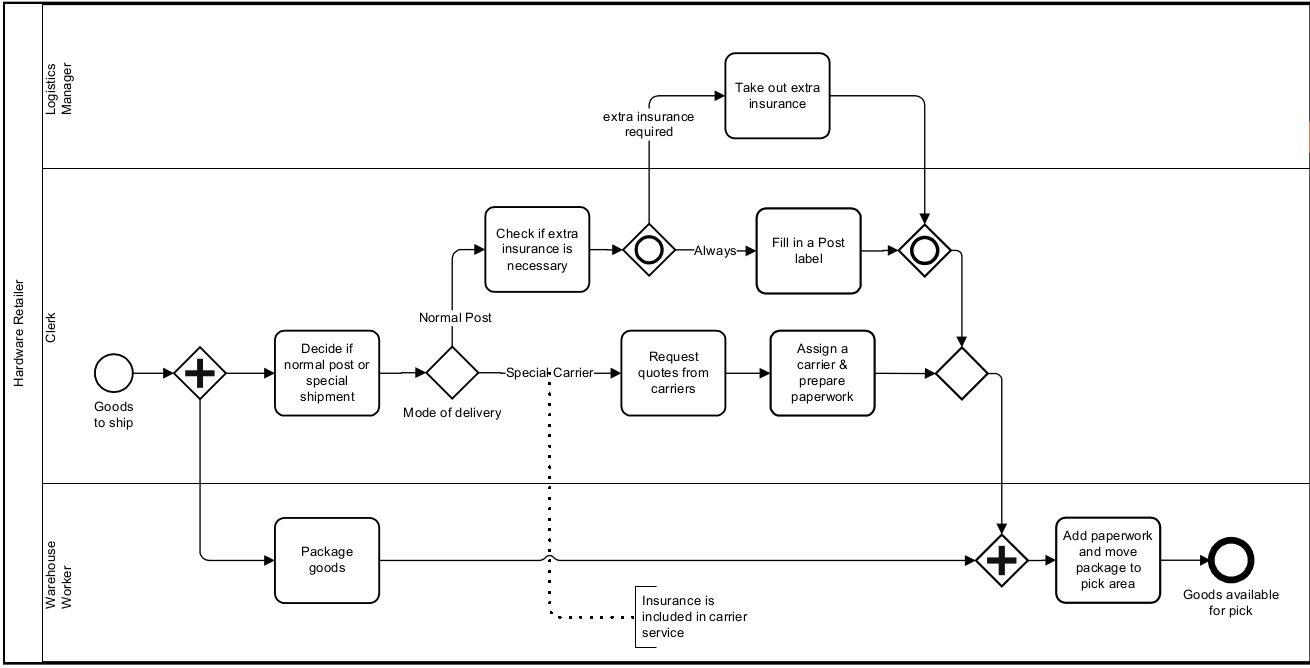
\includegraphics[width=0.85\textwidth]{BPMNex.png}
\caption{A simple example of a business process using BPMN from \autocite{BPMNexample}}
\end{figure}

Above is a small example of the BPMN reprensentation of a business process. You can see how clear and straightforward this is. You don't need to understand the BPMN standard or have read the six hundred pages specification to grasp the meaning of this flow chart.

Another reason for using BPMN as a business process modelling tool is the Apromore a java API already developed that allows us to store, represent and compute models of business processes. Furthermore Apromore is a mature, well written library that facilitates the management of large business processes and models. It also includes a presentation part which is integrated with graphiti (the eclipse plug-in library for presentation) in Regorus. With this library we can use only one memory model for business processes from graphical specification to compliance checking. \autocite{ApromoreWebsite}



\subsection{An algorithm for business process compliance}
In the previous sections we described the framework used to express laws and regulations in a proper logical way. We also presented BPMN 2.0 as a way to graphically represent business models. Now that we have a standardized formalism on both sides we can put them together and let the magic happen. In the following we will present the business process compliance algorithm as it is implemented in Regorus and as featured in \autocite{ConceptuallyRichModelofBPC}.

For a given business process the algorithm starts by computing all the possible traces, all possible executions of the business process. In order to do so a reachability graph is computed first using the method described in \autocite{sweepline2004}. From this are drawn all possible executions of the process. 

Now that we have all possible traces we will focus on one. For each task in the trace several actions are accomplished. First a call is made to the rule engine with the informations about the task. It will return the new obligations generated by these antecedents. These new rules are added to the Current set which contains all rules in-force at a given task. We consider $C$ as an \ochain of obligations $C= B_{1} \otimes B_{2} \otimes A_{1} \otimes A_{2} \otimes$. The Unfulfilled set contains all achievement and maintenance rules that were triggered but not fulfilled yet.

The terminated set contains rules that were terminated according to the following definition from \autocite{ConceptuallyRichModelofBPC}. A chain $C$ is terminated by a task n if $C$ was active at task n and that another rule $r$ triggered at task n derives the opposite of $C$. The rule $r$ must not be weaker than the rule that originally yielded $C$.

\begin{algorithmic}
\ForAll{C $\in$ Current} 
	\If{$A_{1}$ = $O^{p}B$}
		\If{$B \in S$}
			\State remove([T,R, $A_{1} \otimes A_{2}$], Current)
			\If{[T,R, $B_{1} \otimes B_{2} \otimes A_{1} \otimes A_{2} \otimes$, $B_{2}] \in$ Violated}
				\State add([T,R, $B_{1} \otimes B_{2} \otimes A_{1} \otimes A_{2} \otimes$, $B_{2}]$, Compensated)
			\EndIf
		\Else 
			\State remove([T,R, $A_{1} \otimes A_{2} $], Current)
			\State add([T,R, $A_{1} \otimes A_{2}$, $B$], Violated)
			\State add([T,R, $A_{2}$], Current)
		\EndIf
	\EndIf
	\If{$A_{1}$ = $O^{a,x}B$}
		\If{$B \in S$}
			\State remove([T,R, $A_{1} \otimes A_{2}$], Current)
			\State remove([T,R, $A_{1} \otimes A_{2}$], Unfulfilled)
			\If{[T,R, $B_{1} \otimes B_{2} \otimes A_{1} \otimes A_{2} \otimes$, $B_{2}] \in$ Violated}
				\State add([T,R, $B_{1} \otimes B_{2} \otimes A_{1} \otimes A_{2} \otimes$, $B_{2}]$, Compensated)
			\EndIf
		\Else
			\State add([T,R, $A_{1} \otimes A_{2} \otimes$], Unfulfilled)
		\EndIf
	\EndIf
	
	\If{$A_{1}$ = $O^{m}B$}
		\If{$b \notin S$ or $\neg B \in S$}
			\State add([T,R, $A_{1} \otimes A_{2}$, $B$], Violated)
			\State add([T,R, $A_{2}$], Current)
		\EndIf
	\EndIf
\EndFor

\State

\ForAll{$C \in$ Terminated}
	\If{$C \in$ Unfulfilled}
		\State add([T,R, $A_{1} \otimes A_{2}$, $B$], Violated)
		\State add([T,R, $A_{2}$], Current)
	\EndIf
	\If{$A_{1} = O^{a,\tau}$}
		\State remove([T,R,$A_{1} \otimes A_{2}$], Current)
	\EndIf
\EndFor
\end{algorithmic}



\subsection{Tools already developed : Regorus and SPINdle}

The business process compliance project takes its roots back about five years ago when the first papers were published \autocite{journeyToBPC}, \autocite{isf09compliance}. During this time research in both the theoretical framework and its implementation have been conducting leading today to two main tools : SPINdle the rule engine and Regorus the business process compliance tool. In the following section we will portray both software, their functionalities, their use and what improvement could be made.

\subsubsection{Regorus}
We already mentioned Regorus a few times before but never detailed its functionalities. In this section we will describe what are the main components in it and how they interact

Regorus is a business process compliance suite that contains multiple software providing a complete environment for compliance officers. First, the rule editor that offers a web interface to write defeasible rule. It is very easy to use and provides lots of features (auto-completion, English translation of defeasible rule, etc.) making the rule edition clear and effortless even for people not familiar with defeasible logic. Second, the eclipse plug-in focuses on the business process modelling part. It is possible to create and annotate business processes and check for compliance. It uses the broad APIs of eclipse for graphical modelling and the Apromore library to integrate BPMN 2.0 shapes. Finally the core library is where the business part is happening. It has multiple point of entry for the other software in the suite to interact with it. It offers a complete and comprehensive list of functions for business process compliance checking.

Regorus is a complex software written in Java and using multiple third-party libraries. It is hard to get a global understanding of all its components. Some of the external libraries don't get much support or are breaking their APIs leading to an ever ending effort of keeping the software up to date with the major releases. This contributes to the complexity of Regorus especially when trying to build it from source. I will explain in more details the work of porting the eclipse plug-in to the new major release of the Eclipse API in a ulterior section.

Regorus is about to undergo major changes in its core and eclipse plug-in parts to implement temporal defeasible logic in the code. New notations and semantics will have to be added to the code-base. At a smaller level I contributed to the extension of Regorus by implementing cooccurrent obligations in both the core libraries and the rule editor.

\subsubsection{SPINdle}

SPINdle is the rule engine that computes the consequences of a defeasible theory. It derives obligations and facts from literals that can be obtained from annotation on a business process. It is a free software distributed under the GNU general public license and can be used by in any project that want to leverage the power of defeasible logic.  \autocite{spindleUserManual}

SPINdle offers multiple interfaces to interact with it. This allows other programs to rely on this for the logical inference part as we do with Regorus. SPINdle is implemented in Java and therefore integrates mostly with JVM based languages. Although a web-service implementation would increase interoperability with other software it is not an implemented feature yet. 

Theories can be submitted and conclusions retrieved using XML or DFL (a specific formalism to describe theories and conclusions). It also gives interfaces for users interested in implementing their own parsers. Using this loosely coupled setup adds makes the use of SPINdle very agile as when there is a change in regulation you only need to change your DFL of XML file and not touch the SPINdle code.

In the specific use case of Regorus and business process compliance, SPINdle is called to get conclusions at each task of all the traces for a given business process. Consequently, SPINdle is highly optimized using algorithms proposed in \autocite{MaherSPINdle} in versions 1.X.X and an improved version \autocite{LamSPINdle} in versions 2.X.X leading to better performance.

The next major release of SPINdle will include support for temporal defeasible logic. This leads to sizeable changes in the core algorithm computing the conclusions of a theory but also in the input method as it needs to include new notations and semantics.


\newpage
\section{Adding features to Regorus}
\subsection{Implementing Cooccurrent Obligations}
As introduced earlier there is different types of obligation in defeasible logic. This wide range allows us to model precisely and accurately a large number of business processes and rules. However some shortcomings have been spotted leading to imprecise modelling and the need for a new obligation.

\subsubsection{Presentation of the Problem}
Let's first introduce an example to underline the lack of appropriate obligation. Taken from the Australian \textbf{INSERT THE PROPER ACT HERE} act when needing personal information from someone it must be given by the person himself. We could model this rule with a punctual obligation like this :
\begin{equation}
r1 : \text{Need Personal Information} \Rightarrow \text{[Op] Get it in person}
\end{equation}
In the current implementation of the compliance checking algorithm if the effect of the task triggers the rule $r1$ then the obligation is carried on to the next task where it will be checked in the \textit{Current} obligation set. In our example that does not really make sense since once we get the information we should check \textbf{in the same task} is the information was taken personally or not.

To be able to precisely describe this kind of behaviour we need to introduce a new type of obligation, Cooccurrent Obligation. This represent an extension of punctual obligation which must be fulfilled in the same task where it was triggered. The addition of this new obligation forces us to modify the implementation of the software in the core packages to check compliance as well as in the editor part to let the user add this kind of obligation to their implementation of rules.

First let's see how this new type changes the core compliance checking algorithm :

For now the compliance checking algorithm works in five main steps for each task of the business process :
\begin{enumerate}
\item Get the obligations generated from the previous task
\item Get the effects of the current task
\item Generate new effects
\item Check compliance with the given obligations and effects
\item Generate the new obligations for the next task
\end{enumerate}

We need to make a few changes to take into account the new type of obligation. First, in the generated obligations look for Cooccurrent obligations then check these obligations on the literals just generated and see if there is a violation. If this is the case then the chain of reparation is marked as activated and checked for compliance in the task.

As we said before cooccurrent obligations are close relatives of punctual obligations this allows us to leave the compliance checking algorithm and related routines unchanged and just call it again with the freshly generated cooccurrent obligation as punctual obligations and the new effects. To sum up we add three new steps to the pseudo algorithm introduced previously :
\begin{enumerate}
\item Get cooccurrent obligation from the set of new obligations
\item Call the compliance checking algorithm to check compliance with the new effects and the cooccurrent obligations
\item Generate new obligations for the next task and forward
\end{enumerate}

Now we need to take into account violation and compensation. If a cooccurrent obligation is violated and if it is part of a compensation chain we will check the rest of the chain in the very same task it was activated.

\subsubsection{Implementation in the codebase}

The implementation of the compliance checking algorithm is located in the core library of Regorus in \inlinecode{AbstractSessionImpl.java}. The implementation was fairly straightforward as the existing code was very close to the theoretical algorithm presented earlier. The logic is to identify cooccurrent obligations in the results of SPINdle then put those in the current obligation set so that they are checked in the same task and then add an \texttt{if} statement to handle the cooccurrent logic as explained above.

Also I added cooccurrent obligations to the types of obligations already implemented in \inlinecode{ObligationType.java}. All obligations types are created using a single private constructor : 
\begin{lstlisting}
private ObligationType( final boolean aAchievement, final boolean aPersistent,
                        final boolean aPreEmptive,  final boolean aMaintenance,
                        final boolean aPunctual,    final boolean aCooccurrent,
                        final String aDisplayName,  final String aModeName);
\end{lstlisting}
This constructor only sets the associated fields with the value given in parameters.

Static final shortcuts are provided that return any type of obligation. For example in the cooccurrent case : 
\begin{lstlisting}
public static final ObligationType COOCCURRENT = 
	new ObligationType(false, false, false, false ,false, true, 
                           "Co-occurrent Obligation", COOCCURRENT_MODE_NAME);
\end{lstlisting}

Is also featured some helper functions that had to be modified to include cooccurrent obligations. These are : 
\begin{itemize}
\item \String identifiers for different types of obligation (\inlinecode{"0C"} for cooccurrent, \inlinecode{"OANPNP"} for non-persistent, non-preemptive achievement obligations, etc.),
\item An array of \String containing all the obligation modes names
\item \inlinecode{public static ObligationType fromModeName(final String aModeString)} which returns an obligation from the \String representing the obligation's mode.  
\end{itemize}

Changes were also made in the rule editor to be able to create rules using cooccurrent obligations. I added cooccurrent obligations to the auto-completion feature so that this new type is proposed to the user when drafting rules. I also added cooccurrent obligation in the part that interfaces with the core library of Regorus. The work done was mostly, as shown above, searching how features were implemented, understand the algorithms and add the new type of obligation. This was not an easy task since multiple programming languages were involved (Java, Groovy, JavaScript, Scala). I had to adapt to very different situations and train myself on these languages in order to gain a basic understanding of them.



\subsection{XOR splits and the condition associated to them}
In order to be able to implement conditional splits in business processes it is necessary to have XOR splits and corresponding XOR join. Unfortunately with this mandatory tool for business process modelling comes some issues, especially with punctual obligations, that we will try to tackle.

First let see how XOR nodes behave in business process modelling with a little example from a demonstration video of Regorus \autocite{regorusVid}.

\begin{figure}[!h] %on ouvre l'environnement figure
\begin{center}
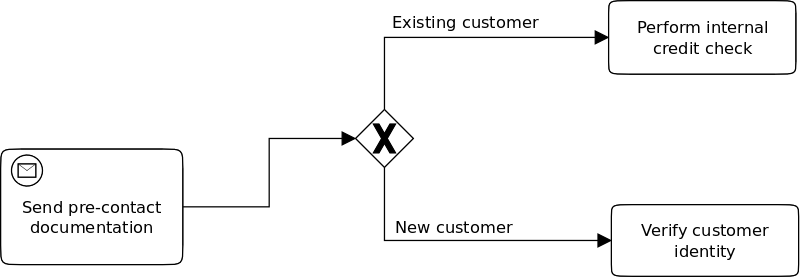
\includegraphics[height=3.4cm]{XOR.png} %ou image.png, .jpeg etc.
\caption{A simple example of XOR split} %la légende
\end{center}
\end{figure} %on ferme l'environnement figure 

This sample shows an important feature of the XOR nodes : annotations on the edges. When checking compliance all the possible executions of a given business process are computed which mean in one case we will have \textit{Existing Customer} as an effect and in another thread we will have \textit{New Customer} as effect. The issue is in the way we take these effects into account to check compliance in the following tasks.

For now Regorus puts \enquote{dummy nodes} between the XOR split and the first task as shown in the following illustration.
\begin{figure}[!h] %on ouvre l'environnement figure
\begin{center}
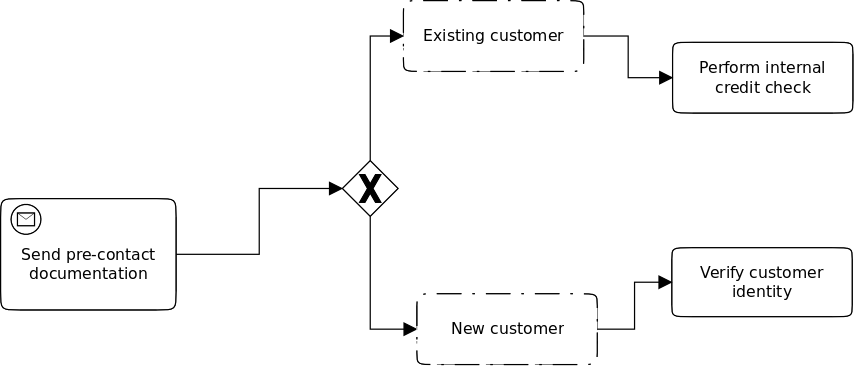
\includegraphics[height=4cm]{XOR2.png} %ou image.png, .jpeg etc.
\caption{Illustration of the \enquote{dummy nodes} added by regorus} %la légende
\end{center}
\end{figure} %on ferme l'environnement figure

But a better behaviour would be to take these directly into account without the need for dummy nodes. Indeed punctual and cooccurrent obligations cannot be handled properly in this case. If the node before the XOR split yields an punctual obligation like this one $\text{p} \rightarrow \text{[Op]q}$ then with the actual implementation the obligation will be checked in the dummy nodes when it should be checked for compliance in the first \enquote{real} node following the XOR split.

Again for cooccurrent obligations if the effect associated with the edge of the XOR split yields a cooccurrent obligation like $\text{p} \rightarrow \text{[Oc]q}$ then it will be checked on the dummy node when it should, once again, be checked for compliance in the first \enquote{real} node following the XOR split.

We chose to follow these steps to implement this desired behaviour :
\begin{enumerate}
\item Identify the XOR splits in the business process graph
\item When on a XOR split make a call to SPINdle to generate the obligations triggered by the effect associated with the edge,forward the new obligations to the next node without calling the compliance checking algorithm
\end{enumerate}

\paragraph{Just Thinking about stuff} 
So if XOR splits conditions are not implemented in the code, how are they taken into account. I think they are put in by the eclipse plugin maybe using some special apromore feature. If that is the case we need to see if it translates to a kind of dummy task. How is that implemented in the core library. Wouldn't it be better if the core library could handle that rather than leaving this to the eclipse plug-in ?


\subsection{Porting the eclipse plug-in to the Kepler version of Eclipse}

New releases come with their burden of broken APIs and unresolved functions names. Eclipse is not an exception for that matter. The Eclipse plug-in code has not been touched for two years so when I tried to compile and run it on my machine I stumbled upon a lot of errors. Like other complex software the eclipse plug-in depends on some third-party library to work properly. These evolved quite a bit over time to a point where function that once existed where not even referenced in the last version.

First let me tell you about the \textit{graphiti} library. It's a component of the \enquote{Eclipse Modelling Framework}. As one of the main feature of the plug-in is to be able to draw business process, it relies on this library. Really this hasn't been too much of a hassle since like other eclipse core libraries it is pretty well documented and the javadoc is easily available online. One of the methods the code was using wasn't referenced any more in the Kepler version of the library and the type calling this method was marked as deprecated. 

I eventually found a workaround for my problem but it taught me a great lesson for future software documentation I may write : always not only document what you changed but also why or to what purpose you changed the library.

This task also trained me on a part of software development we rarely talk about in class : production environment and dependency management. Developing a software that is portable is really important and it must be a very important concern. Will the libraries I use be available for future developers ? Are the maintainers of these libraries care about backports or keeping legacy software usable ?
These are very important concerns and even more difficult to enforce in a Java environment. %citation needed


\section{Extending the theoretical model by adding time}

We have seen before that obligations in regulations are often closely related to the notion of deadlines for example the obligation \textit{Pay before ten days} holds a deadline information. Defeasible Deontic Logic with BPMN 2.0 as implemented in Regorous is a powerful tool to deal with business process compliance. However defeasible deontic logic does not handles time and deadlines by design. Sure it is possible to use facts as ersatz for time for example the rule introduced before can be modelled as : $r: \neg \text{moreThan10Days} \Rightarrow O_{a}Pay$ and this could translate in a task of the business process having the literal $ \neg \text{moreThan10Days}$ attached but there is room for improvement.

\subsection{Motivation for adding time in defeasible logic}

Adding time in defeasible deontic logic is a much anticipated feature because it implements at the source the essence of deadline allowing us, as we will see later on, to represent obligation types elegantly. In \autocite{TemporalExtension2007} extensions to include time in the logic are proposed and we will use these semantics and notations.

Moreover time in the framework is expected to improve the computational efficiency of the system. For now we check compliance at each task of the business process collecting the new rules and forwarding them to the next task. With time we could do all of this at once. With temporal rules we would only need to create traces which would yield a set of temporal literals and check this set against the set of temporal rules. Let's take the following little example : 

\begin{figure}[!h] %on ouvre l'environnement figure
\begin{center}
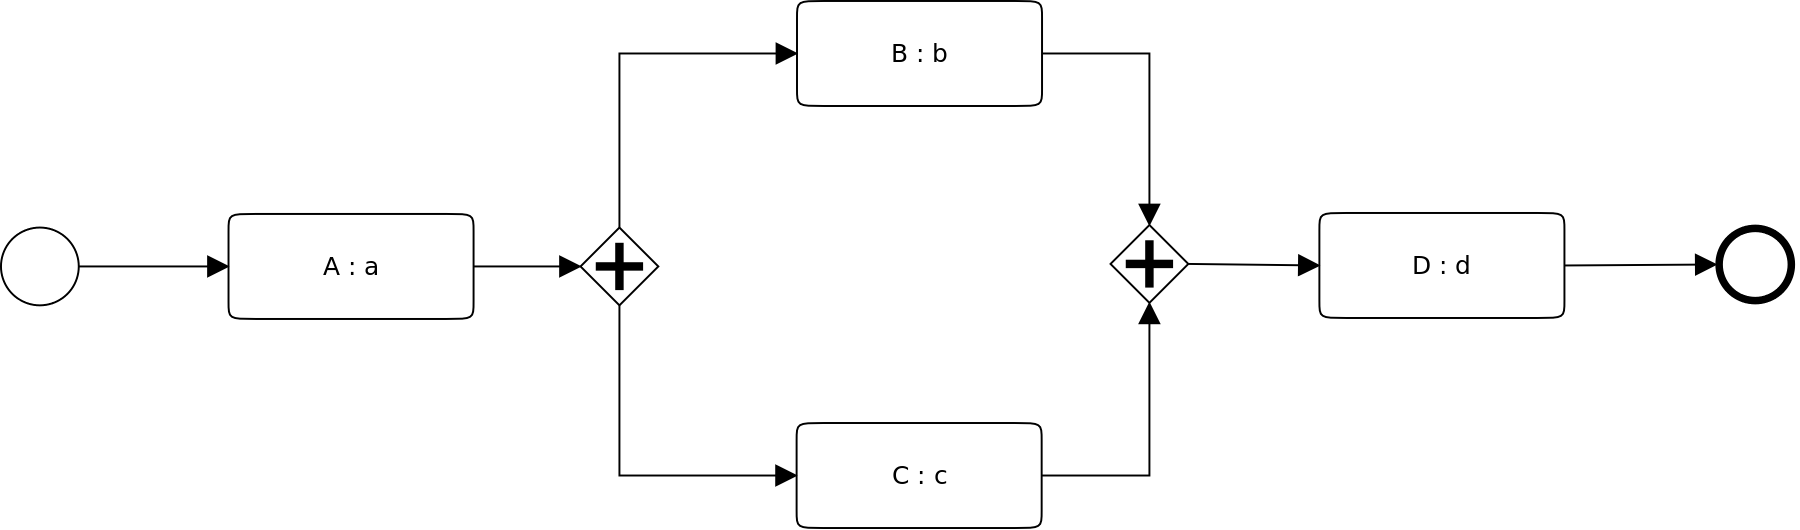
\includegraphics[width=0.85\textwidth]{temporalExample1.png} %ou image.png, .jpeg etc.
\caption{A simple Business Process example to highlight the advantages of adding time} %la légende
\end{center}
\end{figure} %on ferme l'environnement figure

For this example we would first compute all the possible traces which gives us two possibilities either $A \rightarrow B \rightarrow C \rightarrow D$ or $A \rightarrow C \rightarrow B \rightarrow D$. Now that we have linear processes we go though each task, accumulate effects, derive rules in force, check for compliance and then forward effects and obligations to the next task. For a trace of size $n$ we have to do each operation $n$ times.

If we add time though, we only need to do the computation once for any process size, this is a huge win for scalability. This time we can annotate effects attached to task with the task number in the trace or let the user use its own annotations, we then go through the process once to accumulate all the effects, finally we check compliance against temporal rules using temporal defeasible logic.

%how adding time liberate us from doing this? need a clear example and maybe some images.

\subsection{Temporal formalism for deontic defeasible logic}

\autocite{JusticeDelayed2011} introduces new notations, semantics and concepts to deal with time in deontic defeasible logic. They represent time as a discrete linear order of instants $ \mathscr{T} = (t_{1}, t_{2} ... t_{n})$.

The following list sums up the notations introduced in \autocite{JusticeDelayed2011} and their semantic :
\begin{itemize}
\item if $l$ is a literal then $l^{t}$ is a temporal literal. We will refer to the set of temporal literal as $\text{TLit}$. We also introduce $\top$ and $\bot$ which are also temporal literals, they are propositions that are respectively always complied with and never complied with
\item if $l^{t}$ is a temporal literal then $Ol^{t}$ and its negation are deontic literals meaning that the obligation to do $l$ holds at time $t$. We will refer to the set of deontic literals as $DLit$
\item if $a^{t_{a}}$ and $b^{t_{b}}$ are temporal literals, $t \in \mathscr{T}$ and $x \in \{a,m,p\}$ then $a^{t_{a}} \otimes^{x}_{t} b^{t_{b}}$ is an \ochain used to express chain of reparation in laws
\item if $\alpha$ is an \ochain, $t$ and $t_a \in \mathscr{T}$  and $a^{t_{a}}$ is a temporal literal then $\alpha \otimes^x_t a^{t_{a}}$ is an \ochain . A deontic expression is an \ochain\ composed of temporal literals or sub-\ochain and finishing with $\bot$
\end{itemize} 


An \ochain like $\alpha \otimes^{a}_{t} a^{t_{a}} \otimes^{y}_{t'} b^{t_{b}}$ means that the violation of $\alpha$ triggers an achievement obligation from $t_{a}$ to $t'$.

Temporal defeasible logic also defines new defeasible proof conditions. \ref{def-temporal-applicable} shows when a rule is applicable at index $i$, meaning that the obligation at index $i$ in the \ochain\ is in force.

\begin{mydef} \label{def-temporal-applicable}
A rule $r$ is applicable at index $i$ in a proof $P$ at line $P(n+1)$ iff
\begin{enumerate}
\item $\forall a \in A(r)$
      \begin{enumerate}
      \item if $a \in \mbox{TLit}$, then $a \in F$ and
      \item \begin{enumerate}
            \item if $a = Ol^t$ then $+\partial l^t \in P(1..n)$
            \item if $a = \neg Ol^t$ then $-\partial l^t \in P(1..n)$ and
            \end{enumerate}
      \end{enumerate}
\item $\forall c_j \in C(r)$, $1 \leq j \leq i$
      \begin{enumerate}
      \item if mode($c_j$) = punctual, then $c_j \notin F$ or $\sim c_j \in F$
      \item if mode($c_j$) = achievement, then $\forall t$, start($c_j$) $\leq t \leq$ end($c_j$), $c^t_j \notin F$ or $\sim c^t_j \in F$
      \item if mode($c_j$) = maintenance, then $\exists t$, start($c_j$) $\leq t \leq$ end($c_j$), $c^t_j \notin F$ or $\sim c^t_j \in F$
      \end{enumerate}
\end{enumerate}
\end{mydef}

In \autocite{JusticeDelayed2011} different proof conditions are defined for each obligation type. In \ref{def-temporal-proof} we present them in a condensed form. $x$ is used to represent the mode of the obligation, it can be replace by one of ${a,m,p}$.

\begin{mydef} \label{def-temporal-proof}
If $P(n+1) = +\partial p^t$ then
\begin{enumerate}
\item $\exists r \in R^{x}_{\Rightarrow}\left[p^t,i\right]$ , $r$ is applicable at index $i$
\item $\forall s \in R[\sim p^t, j]$ either
      \begin{enumerate}
      \item $s$ is discarded at index $j$
      \item $\exists w \in R^{x}_{\Rightarrow}\left[p^t,k\right]$, w is applicable at index $k$ and $w\succ s$
      \end{enumerate}
\item $\exists x \in R^{a,m}_{\Rightarrow}\left[p^{t'},i'\right]$, $t' < t$, end($t'$) $\geq t$
      \begin{enumerate}
      \item $x$ is applicable at index $i'$, and
      \item $\forall y \in R\left[\sim p^{t''},j'\right]$, $t' \leq t'' < t$ either
            \begin{enumerate}
            \item $y$ is discarded at index $j'$ or
            \item $\exists z \in R\left[\sim p^{t''},k'\right]$, $z$ is applicable at $k'$ and $z\succ y$; and for $+\partial^a$
            \end{enumerate}
      \item $\forall t'''$, $t''<t'''\leq t$, $p^{t'''} \notin F$.
      \end{enumerate}
\end{enumerate}
\end{mydef}

Conditions (1) and (2) are enough to defeasibly prove a punctual obligation. (3) only applies for maintenance and achievement obligations. The final line (3.c) only applies to achievement obligations where fulfilment terminates the obligation.

\subsection{Proving that defeasible logic and temporal defeasible logic reach the same conclusions}

It is important to prove that given the same process and rules both versions of defeasible deontic logic with and without time reach the same conclusions about compliance. This allows us to confidently move on to the implementation of the compliance checking algorithm in temporal defeasible logic.

A defeasible theory is defined by the tuple $(F, R, >)$ where $F$ is a finite set of literals, $R$ a finite set of rules and $>$ a superiority relation on $R$. In the context of business process compliance we consider $S_{1}..S_{n}$ sets of literals representing the literals attached to every task. Therefore for each task we have a different theory. At task $n$ we have $F = \bigcup \limits _{i=1}^n S_{i}$, the set of rules stays the same although the obligations in force can change from one task to another.

A temporal defeasible theory is not so different from its classical counterpart. It is defined by the tuple $(F^{t}, R^{t}, \succ)$ where $F^{t}$ is a finite set of temporal literals, $R^{t}$ is a finite set of temporal rules and $\succ$ is a superiority relation on $R^{t}$. The Facts and Rule sets are dependent of the current task in a given trace. We highlight this dependence in the following.

We are defining the $\tempop$ operator which takes a defeasible theory and a point in time and returns the temporal equivalent, formally defined as : 
\begin{gather}
\tempop : \mathbb{N}, (F, R, >) \rightarrow (F^{t}, R^{t}, \succ)
\end{gather}

Every literal in $F$ is temporally annotated with the task number it is attached to. We know that at a given task F is the union of the previous $S_{i}$ therefore at a given task $t$ we have. 

\begin{gather}
F^{t} = \{q^{t} \quad | \quad \forall q \in S_{t} \}
\end{gather}

Every rule in $R$ is translated by annotating temporally with the current task number all its antecedent and consequent. The temporal rule arising from a classical rule depends on the task number in a given trace. For each task in every possible trace we define a set of temporal rules corresponding to the body of \enquote{classic} rules. All of the antecedents and effects of the rules are annotated with the task number which will play the role of time as the set of task numbers is isomorphic to $\mathbb{N}$ which is a perfect candidate for time. Since defeasible deontic logic does not include deadlines we transform achievement and maintenance obligations to permanent ones defining an \enquote{infinite} deadline and we translate punctual one with a deadline set to the next task.

Let's introduce the mode function that returns the mode of a given obligation :

\begin{gather}
mode(O) = \begin{cases}
a & \text{if $O$ is an achievement obligation}\\
p & \text{if $O$ is a punctual obligation}\\
m & \text{if $O$ is a maintenance obligation}\\
\end{cases}
\end{gather}

Here we will show how the set of temporal rules $R^{t}$ is derived from the set of classical rules $R$. First in \ref{defGeneralRule} we define a general form for classical rules we will use to define how we translate to temporal rules.

\begin{equation} \label{defGeneralRule}
\forall r \in R, \quad r :  a_{1}, ..., a_{n} \Rightarrow p_{1} \otimes ... \otimes p_{m} \\
\end{equation}

Let me introduce in \ref{defNuf} one of the tools we will need for this demonstration the $naf$ operator. It stand for negation as failure which means that we failed to prove an element. It is defined practically as : 
\begin{equation}\label{defnaf}
\begin{aligned} 
&r_{1} :& &\Rightarrow naf\,p \\
&r_{2} :& \neg p &\Rightarrow naf\,p \\
&r_{3} :& p &\Rightarrow naf\,p \\
& & &r_{3} > r_{2} > r_{1} 
\end{aligned}
\end{equation}

In other words we have $naf\,p$ either when $p$ has not been concluded or $\neg p$ has been concluded. If $p$ is concluded then this rule is stronger than the other two and we conclude $\neg naf\,p$

For demonstration purposes we introduce in \ref{defViol} the $viol$ function which takes an obligation and returns the index of the task where it was violated. If the obligation is never violated it returns the index of the last task. This will allow us to express chain of reparation from the classical framework where no deadlines are defined into the temporal one where we need deadlines. This $viol$ operator will create artificial parametrized deadlines for chain of obligations as it will be presented next.

\begin{equation}\label{defViol}
\begin{split} 
viol(X) : Obligations \rightarrow \mathbb{N}\\
\end{split}
\end{equation}

\begin{itemize}

\item For a maintenance obligation $O^{m}p$, $viol$ will return the index of the first task where the obligation is applicable and we can conclude $naf\,p$. 
\begin{equation} 
\begin{aligned}
& \text{At task i if we have : } O^{m}p \text{, } naf\,p \in Facts\\
& \text{then : } viol(O^{m}p) = i\\
\end{aligned}
\end{equation}

\item For an achievement obligation $O^{a}p$, $viol$ will return the index of the first task where the obligation is applicable, we can conclude $naf\,p$, and the obligation is lifted at the next task (this can be done with defeaters).
\begin{equation} 
\begin{aligned}
& \text{At task i if we have : } O^{a}p \text{, } naf\,p \text{, } \neg O^{a}p \in Facts\\
& \text{then : } viol(O^{a}p) = i\\
\end{aligned}
\end{equation}

\item It is not necessary to define $viol$ for punctual obligations since they are always violated or fulfilled at the task after they were triggered. For example $O^{p}p$ is triggered at task $i$ then it is either complied with or $viol$ will return $i+1$.
\end{itemize}


Now we will show how we translate temporally each of these rules, given a classical rule $r$ in the form defined in \ref{defGeneralRule} at a given task $t$ the set of temporal rules is composed of rules.

\begin{equation} \label{ruleClassicToTemp}
\begin{aligned}
&r_{i} :& a_{1}, ..., a_{n} &\Rightarrow p_{1} \otimes ... \otimes p_{m} \\
&r_{i} (task) :& a_{1}^{task}, ..., a_{n}^{task}  &\Rightarrow^{mode(p_{1})} p_{1}^{task} \otimes^{mode(p_{2})}_{viol(p_{1})} p_{2}^{viol(p_{1})}  ...      \otimes^{mode(p_{m})}_{viol(p_{m-1})} p_{m}^{viol(p_{m-1})} \otimes \bot
\end{aligned}
\end{equation}

\paragraph{Consider sets of obligations from the algo}
Now we are considering the sets of obligation we find in the algorithm for business process compliance checking. In this we find at each task three main sets of obligations and literals : Current, Violated and State. They contain respectively obligations in force at the given task, obligations that were violated in previous tasks and deontic literals attached to the current or previous tasks. We aim to prove that the transformation of these sets from \enquote{classical} formalism to temporal is isomorphic and our transformation bijective. All these set are depending on the current task we consider, they will be referred as : $\text{Set}(n)$

First let's proove that $$\text{if}\ p \in \text{State}(n)\ \text{then}\ +\partial p^{n} $$
this is trivially proven by definition of our translation where every literal associated with a task is annotated temporally with the task number in the trace. Therefore if $p$ is in the $\text{State}(n)$ it has been proven at a step $(1..n)$.

Now what about $$\text{if}\ q \in \text{Current}(n)\ \text{then}\ +\partial Oq^{n} $$
If an obligation is in force at a task n in the \enquote{classical} formalism is it also in the temporal one, in other word is the rule applicable at the index where it triggers $q$. If $q$ is in the set of current obligation it means that there is a rule $r$ that yields $q$ at task $k$ and that this rule was fired meaning all of the antecedents have been proven. In other words :
\begin{align*}
&\forall a \in A(r),\ a \in\ \text{State}(k) \\
& \text{so if}\ a \text{ is a literal then }   a \in \text{ Facts} \\
& \text{or if } a\ \text{is an obligation } Ol\ \text{then } +\partial l^{1..k} 
\end{align*} 

Or, the conditions on the Antecedents for a rule to be applicable are :
\begin{itemize}
\item if the antecedent is a litteral then it must be in the Facts (attached to a previous task)
\item if the antecendent is an obligation then it must have been defeasibly proven beforehand.
\end{itemize}
Both conditions are met so the rule would also trigger in temporal defeasible logic. Now we have to see if it would trigger at the right index in the \ochain.

If $q=Ol$ is part of an \ochain like $A_{1}\otimes .. \otimes A_{n} \otimes q \otimes B_{1} \otimes .. \otimes B_{n}$ and if $q$ is in current that means that for all obligation $A_{i}$, $-\partial A_{i}$ has been proven for a previous task $(1..k-1)$. Let $m$ be the task where the rule was triggered first. Which translates into :
\begin{itemize}
\item for punctual obligations this means we either have $\neg l$ at task k when the obligation was triggered or that $l$ was not in the State set at task k.
\item for achievement obligations this means that we have $\neg l$ at a task between $m$ and $k-1$
\item for maintenance obligations this means that we either have $\neg l$ at a task between $m$ and $k-1$ or that $l$ was not in the State set at a given task between $m$ and $k$ 
\end{itemize}

Whatever the obligation this means that at some point we were able to conclude $-\partial A_{i}$ for all the obligations before $q$ which means that the rule $r$ is also applicable at the index where it triggers $q$ implying that $q$ is also in the set of Current obligations in the temporal formalism.

We can easily translate this reflection to the Violated set. If a obligation $Ol$ is in the violated set this means that at some task between $1..n$ we have one of the three conditions aforementioned for each type of obligation. Which trivially translates into being able to prove $-\partial l$ at some task $(1..n)$ implying that the obligation is also in the Violated set in the temporal formalism.

We have proved that the sets we have in the algorithm for business process compliance stays the same when we translate a theory from the classical to the temporal defeasible logic. This means that a business process that was (non-)compliant in the classical framework is also (non-)compliant in the temporal one. We have a consistent 

\newpage
\chapter{ Strategic reflection on Regorus}

\section{Business Process Management and Compliance}

Business processes are at the center of any corporation. They have an influence on everything the company produce or services. They model the work of every employee by determining tasks, jobs and responsibilities. A firm that is aware of its processes can adapt faster and painlessly to change in the market or to new regulations. Despite these clear advantages, business processes have been overlooked for a long time by both the academic literature and the businesses. \autocite{dumas2013}

Global markets more competitive than ever, the need to communicate in a scattered market of technologies and the will for any organization to innovate lead to a reflection on the corporate world to try, adjust and optimize the organizations. This ultimately highlighted the importance of business processes and to the creation of Business Process Management to unify and strengthen previous approaches from different disciplines. \autocite{dumas2013}

Compliance is a growing concern for any company, it represents on average 4\% of the annual costs \autocite{IBT2011}. From the same source CEOs of surveyed companies admit that compliance is a major cost centre, that has been expanding in the past years. We are in a situation where businesses have to comply with new regulations that are changing more often. But they are still to find an agile, effective and flexible way to do so. Business process management could help a great deal in this matter. \autocite{goedertier2006}, \autocite{dumas2013}, \autocite{jeston2014}

Revision of regulations is a game changing factor for all companies in a given industry. If we add more flexibility and agility in the compliance world with tools such as Regorus that encourage a compliant by design approach for business processes and provides powerful algorithms to check compliance of existing processes, then, corporations could take advantage of this change in rules to gain a strategic advantage over their competitors.

Also most business don't have explicit business processes when, as we exposed in the previous paragraph, it could help them be more efficient and flexible. We will develop the power of explicit business processes for any institution later when we draw a parallel with knowledge management.Business processes, although often seen as rigid are a real opportunity for any company to be more reactive to change in an always-evolving world.

Finally by releasing companies from the burden and high cost of compliance, money can be better invested especially in innovative activities. Therefore a better management of business processes and compliance contributes to innovation.

Current research is business process management is taking the problem from different angles. A first topic of interest is business process mining where business process management is used as an intelligent IT system. Business processes are automatically generated from the ever-growing data generating from working businesses. From these explicit processes researchers are working on intelligent systems that would give guidelines and propose optimizations of these processes. \autocite{keynoteBae} presents a concrete example of how processes can be improved by these techniques. Of course to express all these processes, powerful, efficient modelling languages are needed and this is another subject of research. Finally the field in which I conducted this project, compliance, is making sure that processes are compliant with regulations with the advantages mentioned earlier.


\section{A critical summary of the work done}

\subsection{Historic}
In this section we will aim to summarize previous attempts to commercialize Regorus and to penetrate the compliance market. Multiple opportunities have presented themselves but non of them have succeeded yet. For each of them we will briefly expose the strategic decisions that were made and expose areas for improvement. Though, we will not cite any names for confidentiality reasons.

Since the product was ready for production use in mid 2012, several companies have expressed an interest in integrating regorus in their compliance teams. Unfortunately, all these attempts have failed so far. In the following section we will present the previous tries to market Regorus and for each of them try to understand what failed and what are the key strength of Regorus from a business point of view.

The first and real contact was with an Australian telecommunication company (later referred as telco). The telecommunication business in Australia is very large. There are more than 2000 firms ranging from Vodafone or Optus who are huge businesses that reach 95+\% of the population to small service providers or system integrators that have 20 or so clients. All these businesses are under the obligation to comply with regulation written by Communication Alliance and enforced by Communication Compliance under the supervision of the Australian Communication and Media Authority.

If Communication Compliance finds a business that is not compliant then it can be put under the scrutiny of the ACMA and be fined or even have its license removed. Therefore compliance is a serious matter for telcos in Australia. The biggest ones are required to be audited by a private third-party auditor when the smaller ones have to ensure compliance by themselves. This is a hard task with very little help from the compliance body apart from some spreadsheets. Thus lot if not all telcos are operating in a grey area where they do not know if their processes are compliant or not, most of them don't even have explicit processes.

A medium size telco CEO visiting a NICTA showcase interested in a compliance system to make up for this less than ideal system. After a demonstration of Regorus she was convinced enough to ask for a trial in her company. The trial was organized around three workshops. The first one was a presentation of Regorus and the underlying theory. The audience was composed mainly of people from the complaint department. Although it was the first time they were exposed to this kind of software the reception was good. The second workshop was focused on helping the staff to model their current processes as they were. In the meantime people at NICTA were implementing a subset of the regulation regarding complaints to check the processes against. During the third and last workshop compliance of processes was tested and yielded interesting results. Some errors were due to incorrect annotations, implementation errors but it also revealed some compliance issues where a redesign of the process was needed.

This workshop was a great opportunity to showcase the power of Regorus on the very same processes these people were working on. This training was a fast and effective introduction, in only three afternoons they were able to understand the basics about the software, how to model their processes and check compliance. These meetings were another indicator that the technology was ready to be shipped into production environment. It also showed that the software was usable by end users with no prior experience with that type of application, they were able to annotate processes, check for compliance, understand the informations and errors thrown at them, etc.

On a strategic point of view it seems that the end users are particularly interested in the product and that the set-up cost is low, only three half-day seminar were enough to launch a team and teach them how to use the product. Although it is hard to conclude anything from one point of data, it seems fair to say that the low set-up cost is an advantage for the product penetration. 

After that, a decision was pending from the certification body, communication compliance, to use Regorus as the compliance checking tool for all small to medium telcos, this represents 90\% of the market in number and around 20\% in value \autocite{telcoIndustryStats}. This was a great idea to target a certification body and have our product advertised by them or even more in that case, a mandatory use of the product. Indeed, the system used at that time was obsolete, it consisted of simple questionnaires on excel spreadsheets to be filled by all telcos. This is a reactive method far from the proactive, compliant-by-design approach of Regorus. Once again, the people who would be actually using Regorus on a regular basis were very happy with the software and were pushing for its adoption. They were also tired and rejected the actual system.

At this point everything seems good for Regorus, end-users are happy with the product, the technology is ready, present systems are obsolete and far less effective than ours and end-users are craving it.

Unfortunately the final decision from the certification body was a no go. The reason given by Communication Compliance was that they were not willing to invest time and money in training all the telcos. I think that one strategical mistake was made here. Instead of targeting the decision makers in the company, it was end-users that NICTA tried to seduce hoping that adoption from them would pressure decision takers. This kind of strategy might work in a technological or research environment where end-users have more skills than the managers and therefore are trusted for decisions concerning the use of one's product. But in this case, even though we had a great success with the end-users and even with their direct management, the real decision makers were not satisfied as they have very different objectives. The question is how to seduce, convince these people to change for our software ? We will discuss this further in the section dedicated to market penetration.

After the telcos, a few other contacts were exploited but lead to nothing concrete. Until a big Australian insurance company showed interest in Regorus. A few meetings were organised with the people on the field, that would actually use the software. Once again, they were very interested in it, saying that it would save them a lot of time and solve some of their problems. However when NICTA asked for a few man-hours to conduct trainings like it had been done with the telco, the upper management refused to. The height of all this is that this very company was fined tens of millions of dollar for non compliance by the regulation authority a few weeks after this.

Lastly, an important consulting firm also showed interest in Regorus and was given an instance to play with. 

\subsection{Comments}
A lot of thinking have been put into this. I found on the intranet lot of documentation from the dev team to try and find possible customer, competitors and strategies. What is missing ? (right person to target) Also working in a very different environment than the technological world. Need to adapt. Need to seek advices from people in this sector (marketing study).


\section{Find a business model for Regorus}

As discussed above, private companies have been keen in the past on integrating Regorus in their processes. Unfortunately it never went through approval from key person in the companies. In the following section we will try to find in which existing business model Regorus could fit and what are the side effects of its use in an organisation. First we will look into Two-sided markets then we will explore how good Regorus is as a knowledge management tool.

\subsection{Two-sided markets}
On two sided market the main sources are \autocite{ParkerA05} \autocite{eisenmann2006strategies} \autocite{rochet2003platform} \autocite{Hagiu2011} \autocite{economides2006}

Which business model ?\\
Who are the clients ?\\
Who are our concurents ?\\

Will the market is likely to end up in a winner take all situation ?\\

Two sided markets are found in many industries but they are particularly found in the high-tech industry. As this market is a high growing one two-sided markets have drawn, over the past decade, a particular interest from researchers in strategy and economics \autocite{Hagiu2011}. In the following section we will first try to come up with a definition of two-sided market or platforms, then we will discuss how Regorus can fit this model. Indeed, Regorus in its essence is a tool that unites different business (law, BP management, IT) therefore it seems quite straightforward that this model could fit it. In a last part we propose different actors that could interact around our platform and unfold strategies following from these hypotheses.

\subsubsection{A definition for two-sided market and its dynamics}

Although there is an extensive literature on the matter a precise definition is yet to emerge. It is not the purpose of this document to propose yet another one, we will try to identify key features of such a market in existing definitions and evaluate their relevance.

First, let us start with a definition from \autocite{Hagiu2011}, that defines multi-sided platforms as : \enquote{An organization that creates value primarily by enabling direct interactions between two (or more) distinct types of affiliated customers}. This definition shows us the two main things to sort out in a multi-sided platform,defining the customers and the kind of interaction they have. 

%\paragraph{Network effects}
Interactions and dynamics in multi-sided platforms are far from the traditional businesses. Here a new kind of complexity is involved : Networks effects, meaning non linear behaviour. Usually the value one side of users attach to the platform depends on the number of users on the other side. This is called \textbf{cross-side network effect}. This effect can be either positive meaning that more users on one side will attract more people on the other side or negative meaning more people on one side decreases the attractiveness of the platform for the other side. Cross side effects can be positive in both way creating a positive feedback on the system (more users on one side attracts more user on the other side that attracts even more user on the other side). In such a configuration the main concern for the platform provider is to reach the critical mass, the tipping point from where the number of user on both side will grow by itself. \autocite{eisenmann2006strategies} This is the case for Groupon where the more customers join the website, the more attractive it becomes for sellers and a great number of deals is an incentive to attract more customers, and so on. However in some cases cross-side network effects are positive in one way and negative the other way meaning that the size of one group of users increases the attractiveness of the platform for the other whereas the size of the latter decreases the attractiveness for the former. In this case the system will reach a dynamic equilibrium at some point. An example would be newspaper where the more readers attracts more advertisers but too much advertisement drives away readers. \autocite{ParkerA05}

There is another network effect in multi-sided platforms \textbf{same-side network effects}, it is the equivalent of cross-side effects but on one side of the platform. An example a positive same-side network effect is Facebook where more users attract even more users as people are keen on joining if their friends are already on the social network website. Unfortunately most of the platform have negative same-side network effects where more people on one side decreases the willingness to join for other users.

%\paragraph{Concerns regarding network effects when creating a platform}
If we forecast positive cross-side and same-side network effects for our platform then the main concern is how to attract the first users to our platform and how many of those do we need to reach a tipping point. We need to find an incentive to make the "penguins jump" \autocite{coursKyle}. Therefore it is important to know what our customers value to be able to give them what they want. As reaching the critical mass is very important in a network environment, knowing the needs and expectations of our customers is a must. 

%\paragraph{Pricing in a platform environment}
Pricing in a platform environment is hard, we have to find a price for each side taking into account the network effects. Usually when we draw demand in function of price we have a linear curve of equation $-ax + b$ but in a platform environment in many cases the demand on one side drops very fast when we go from free to a penny. This is called the penny drop and it is why one side of the platform is generally subsidized. Because the number of users on the subsidized side is highly valued by the other side, the money put into subsidy will be compensated by the price premium we make the other side pay to access our user base. Although most of the classical examples of multi-sided platforms features a subsidized and a money side it is not always the case, if neither sides are money sensitive then we can imagine charging both sides even though one side might be charged less than if we considered a simple-sided classical market.
The objective is to use the network effects and attract money side users therefore we first need to attract the users that the money side users value. And once we attracted these users we need to find the degree of subsidy we will offer to attract enough users and what premium we will charge the other side for the privilege of accessing them. \autocite{rochet2003platform}

%\paragraph{value creation}
An important thing to note is that the value creation in platforms is not in the idea nor in the number of user but in the interaction in the network, the activity of the users. For example twitter idea is worth nothing, just being able to send 140 characters messages through a web application is worthless, its user base is not creating much value either if they don't interact (by tweeting, retweeting, faving other tweets). By doing so they create value for each other \autocite{Choudary2014}. So when looking for a business model for Regorus the quality of the software is not so much relevant. It will at best allow us to make some user jump and hopefully reach the tipping point but the real value of the platform would be the interaction between both sides. How by interacting through Regorous they are creating value for each other. This is an important point that we will consider when looking for solutions to improve market penetration. \autocite{economides2006}

%\paragraph{winner take all}
Because of these non-linear effects, outcomes from multi-sided platform is hard to predict. However history gives us some insight into what we can expect given networks effects in force, multi-homing costs and users sensitivity to new features. Knowing the most likely scenario for the platform tells us if we need to fight to death because we expect a winner take all scenario or to accept competition. The following table gives predicted outcomes depending of the characteristics of the platform :

\begin{center}
\begin{tabularx}{15cm}{|c|p{3.5cm}|X|}
\hline
Likely outcome & Strategy & Platform characteristics \tabularnewline
\hline
Winner Take All & Fight to death & High multi-homing costs on at least one side, Strong positive network effects for the users with high multi-homing costs, Neither side have strong preference for special features.\\
\hline
Cohabitation & Accept competition, Find a niche market & One side at least have special needs, Low multi-homing costs.\\
\hline
\end{tabularx}
\end{center}

Finally some other assets can help to win the war for platform domination \autocite{eisenmann2006strategies} :
\begin{itemize}
\item Pre-existing relations with prospective users on at least one side. This helps at the very beginning when we need to attract early users expecting to feed the positive network effects. It is even more useful if our relation are with influential users in their domain.
\item Reputation can also help a great deal since users are more likely to join if they can put some trust in the platform provider.
\item As we need to reach a critical point for our platform to tip we are likely to subsidize users at the beginning meaning that we could lose money at first. Therefore we will need deep pockets to be able to launch our platform.
\item Because once the tipping point is reached user base will increase exponentially we need to make sure our solution is scalable and wont crumble when stressed with too many requests.
\end{itemize}

\subsection{How does Regorus fits the model}

\subsubsection{Possible users of the platform and strategies}
On one side we have :
\begin{itemize}
\item big firms that already check the compliance of their processes with expensive audits by private firms. They want absolute certainty that this tool will give us reliable results and they want to be able to come back to us if it does not. They don't care about the price because they are already paying lots of money on private audits.
\item smaller firms that are under complex and strict regulations but don't have the money or the manpower to have private or in-house audits for their processes. In this case they probably care a little bit about the price although saying that this might avoid them a big fine might ease things up. We could primarily target firms that were just fined for non compliance.
\item private audit firm could use our software when conducting audits. Because it has already been proven that Regorus is orders of magnitude faster than manually checking for compliance especially when the processes have already been explicited.
\end{itemize}

On the other side we have
\begin{itemize}
\item regulation authorities that probably want the most possible compliant firms in their industry. In the past Regorus have been validated by one regulation agency (the one for telecommunication companies) which is good because we have a clear positive cross-side network effect here, the more regulation agencies saying that our product is yielding good results, creating certified rules to check processes against and especially insuring that the fact that Regorus says it's compliant is equivalent to compliance would be huge. Having a \enquote{marquee user} on one side can attract a lot of users on the other side especially if it states its commitment to our platform \autocite{eisenmann2006strategies}. What could bring user on the other side is if regulation agencies recommend Regorus to firms that have been non-compliant. 
\end{itemize}


\subsubsection{Platform Pricing} 
Since we are considering Business to Business interactions where neither side is money sensitive a subsidy might not be necessary. On the other hand, businesses are extremely quality sensitive and if we want them to integrate Regorus in their processes they need to have some kind of insurance that it will behave correctly especially because we target the compliance world where an error could cost a lot of money. So to make the penguins jump the price is probably not a problem since these companies are already paying good money for private audits of their processes but quality and certification is highly appreciated. Therefore the pricing strategy is not so difficult but need to be though of as this was never properly done before. Once again a study of the market could tell us how much money companies are investing in competitors' software and more broadly in compliance.




\subsection{How Business Process Modelling is integrated in knowledge management}

We think that one of the ways to promote Regorus and improve its market penetration is to research the ways it can be useful for a company. Apart from its main purpose of asserting compliance of business processes Regorus can be useful at higher levels by being a part of the knowledge management plan of the firm.

\subsubsection{Presentation of knowledge management and its advantages}

Knowledge Management is a relatively new field of study born in the early eighties when researchers in management looked into the importance of knowledge in organization.\autocite{Wiig19971}

With the increasing use of information technologies by firms and the escalation in the size of data stored by those knowledge management became a legitimate concern. How to make sense of these ever growing raw databases and extract tangible information out of it? At the same time organization started to consider knowledge as an asset following the lead of Japanese car manufacturers.\autocite{Koenig08} How can a firm use its tacit and explicit knowledge to adapt better to the ever changing market ?

Knowledge management was introduced in popular press in the early nineties mainly through the work of Nonaka. \autocite{nonaka1991knowledge} He is the one who later popularized the concept of Ba in his famous article \autocite{Nonaka_Konno_1998}. In this article he introduces the SECI model aiming to give a framework for knowledge creation within a firm. This model is based on the interactions between explicit and tacit knowledge through four main phases : Socialization, Externalization, Combination, Internalization. Business process explicitation through Regorus editor can be seen as part of the externalization phase where one's knowledge is expressed using the BPMN formalism. Later on this new material can be used in the Internalization phase where this explicit knowledge is used and put into practice as formely formalizes business processes can help in the training of new employees for example.

Regorus is a great tool for companies because it helps them explicit their practices and internal knowledge into a new figurative language such as BPMN. This translates personal, sticky knowledge to be translated into an explicit, normative form leading to a better understanding and transmission of know-how. In this sense Regorous is more than just a tool to check the compliance of processes it is also a powerful way of managing knowledge in the firm and therefore leading to better results.

\subsubsection{Regorus uses BPMN which is designed to make knowledge explicit}
\textbf{ADD THAT BPMN WAS DESIGNED TO INTEGRATE AND EXPRESS BUSINESS PROCESSES}

\section{What can be done to improve market penetration : Qualitative Marketing Research}

As we saw before, a lot of thinking has already been put into strategical reflection for Regorus by the development team. Possible customers and competitors have been identified and the business model have been refined by the previous sections. This is a necessary step in any marketing strategy but it should have been continued by at least a qualitative marketing research to verify if the hypothesis made are right and maybe incorporate new ideas. 

\subsection{Qualitative Marketing Research Explained}

\subsubsection{Definition and Objectives}
Qualitative marketing research main goal is to gather as much information as possible from very different sources, it focuses on the \emph{how} and \emph{why} of the subject under investigation. During the research process it is necessary to adopt an inductive reasoning to build knowledge around what is collected in the different methods put in place. This research method is seeking understanding the reality around marketing and not providing only data without interpretation. \autocite{carson2001}

Qualitative researches can be used to answer questions about \emph{how} and \emph{why} things happen within an organization. They seek a deep understanding of the matter. The profound reasons that lead to a given phenomenon. They are used to uncover the sense behind a \emph{what}. For example a politician may lose 5 points in quantitative polls but it's the qualitative research that will clarify the feelings of the voters. Then another quantitative research can be conducted to see how many people in the population share these perceptions.

\autocite{mintzberg1979} argues that to be effective in real organizations a marketing research must be conducted in the field. It is the very complex and dynamic nature of organizations that make laboratory counterproductive because by simplifying we are excluding the actual thing we should be studying. It is therefore necessary to have contacts with companies and not just only rely on views of the mind.

\autocite{van1979reclaiming} defines qualitative methods as 
\begin{quote}
an array of interpretive techniques which seek to describe, decode, translate and otherwise come to terms with the meaning not the frequency of certain more or less naturally occurring phenomena in the social world.
\end{quote}
This is particularly adapted to our case where we want to understand more about the environment in which decisions are taken in specific markets. It is important that the research is conducted without any judgement with an open mind. We will see that this is a key to have good results and it will be the main focus when conducting focus groups or interviews.

\subsubsection{Interpretation and Reliability of Qualitative Research Results}
We can question ourselves about the credibility of results from qualitative research. After all it is defined as a very subjective methodology and challenges the objective standard of general research results. If another research is conducted will it reach the same conclusions ? Would the theory hold for another environment ? In other word can we generalize it ? These questions can be addressed by following a rigorous methodology throughout the research. The quality of a research is endorsed by three factors : credibility, dependability and conformability \autocite{carson2001}.

The same reference proposes a summary of methods and best practices to generate high-quality results. Some of these methods are applicable to our case. First the persons are chosen not on statistical basis but more on their relevance to the subject under research. Also the interviewing must be deep and intimate to gather interesting results. Furthermore, comparing the results coming from different contexts can help highlight the differences between different user cases. Finally having a feedback on the results of the research from the original respondents can yield interesting results, we could imagine organising a focus group where the original respondents are asked what they think of the research and capture insight on wether they agree or not with the findings of the research.


\subsection{what are we researching ?}
Past experiences and field tests of Regorus have shown two main things. On one hand, end-users are very positive about the software and are able to use it smoothly with very little training. Once set-up it saves them a lot of time and they say they are more efficient in their work. On the other hand, the upper management has always rejected any full-scale tests. The reasons arguing the refusal are mostly \enquote{not enough time}, \enquote{not enough money} or \enquote{we are not big enough}. These were taken as the actual reasons but they are obviously just a quick unthought justification and we think there is more to it than they say. Therefore our first interest will be in finding the actual reason that leads upper-management to reject our project.

Once the \enquote{why} of the refusal is sorted out we can actually try to come up with ideas to bypass these roadblocks. But we think that there is more to that therefore the second interest in our research will try to clarify the decision process of these people. More specifically we will try to identify which incentives they are sensitive to, who are the people they listen to when in doubt, what is important for them.

Finally our last subject of interest is on their expectation for a compliance software such as Regorus. What are the features they like and most importantly why they like it, what are the side effects and improvements they expect by using Regorus and what is their current state of mind regarding compliance software and business process management.



\subsection{The Focus Group (or Interviews), Methodology, Goals and Progress}

Focus groups 

\subsection{Raw Data Analysis : Tools and Methodology}


\paragraph{Methods of Questioning in Focus Group}
What represent the best/worst compliance software ?
What do you expect from it ?


Markets and consumers represent a complex variety of views and perspectives\\
Qualitative market study to discover what our clients are sensible to.\\
Ask questions about the key points presented in the previous section about two-sided networks\\




\newpage
% -------------------------------- %
%           BIBLIOGRAPHY           %
% -------------------------------- %

\newpage

\pagestyle{plain}

% Here is the bibliography on the last page
\nocite{*}
\setlength{\bibitemsep}{5pt}
% \printbibliography[title={Book references},type=book, heading=subbibliography]
% \printbibliography[title={Article references},type=article, heading=subbibliography]
% \printbibliography[title={Online references},type=online, heading=subbibliography]

\printbibliography[title={Technological references},keyword={tech}, heading=subbibliography]
\printbibliography[title={Strategic references},keyword={strat}, heading=subbibliography]

\printbibliography[title={Other references}, notkeyword={tech}, notkeyword={strat}, heading=subbibliography]


\end{document}
